\chapter{Odczytywanie losowego wyniku z kości}

\section{Przetwarzanie wstępne obrazów}

W niniejszym rozdziale omówiono proces przetwarzania wstępnego obrazów kości,
który przekształca dane pochodzące z fizycznego komponentu naszej maszyny (zdjęcia kości) na dane wejściowe dla modelu sztucznej inteligencji.
Przez dane wejściowe dla modelu SI rozumie się tutaj odpowiednio sformatowane obrazy, a więc takie w skali szarości,
o rozmiarach 64x64 piksele, zawierające jedynie kość wyciętą ze zdjęcia całego bębna maszyny.

\subsection{algorytm}

Przetwarzanie obrazów składa się z kilku etapów, które dokładnie opisano poniżej, a workflow prezentuje się tak:
1. Wczytanie obrazu wejściowy \\
2. Odnalezienie kości za pomocą maski na komponencie nasycenia \\
3. Stworzenie i wycięcie prostokąta "Bounding Box" wokół maski \\
4. Przeskalowanie do odpowiedniego rozmiaru \\
5. Konwersja do skali szarości \\
6. Zapisanie gotowego obrazu \\

Na rysunkach <NUMERY> przedstawiono przykładowe zdjęcie surowe oraz poddane już wstępnemu przetwarzaniu.

%% Czy np. dodać elementy pośrednie? - idk

\begin{figure}[H]
    \centering
    \begin{minipage}[t]{0.45\linewidth}
        \centering
        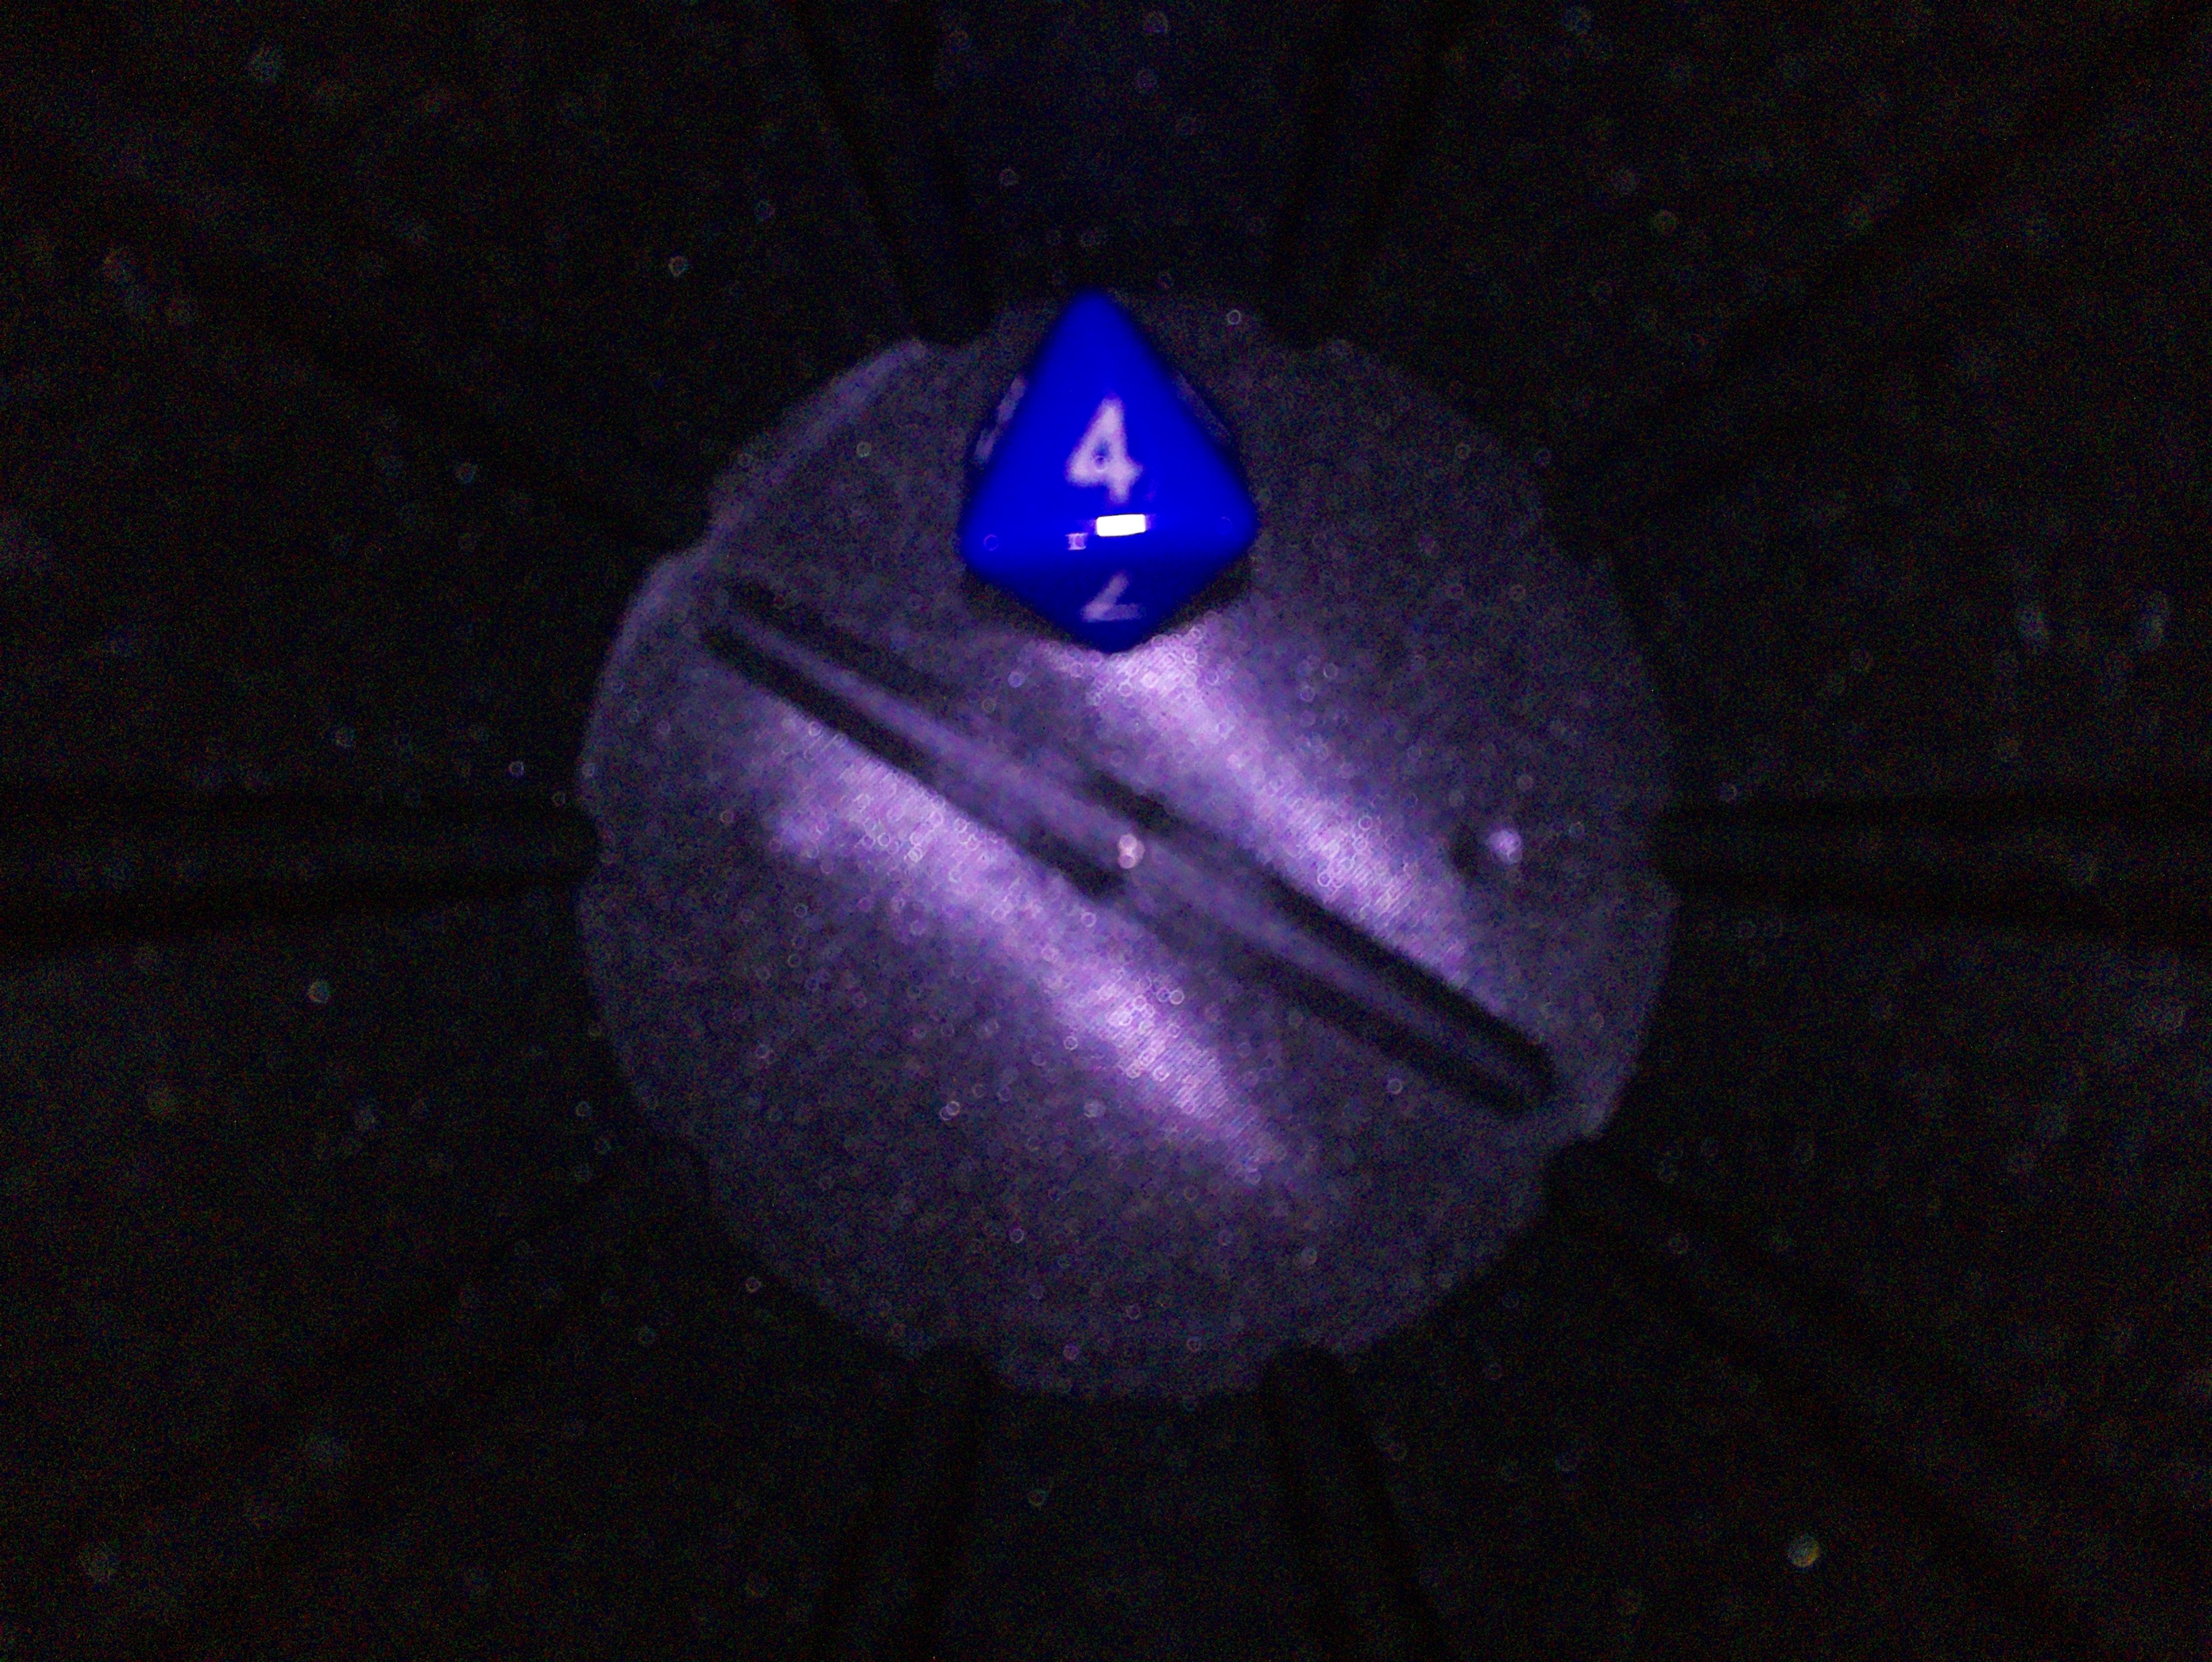
\includegraphics[width=\linewidth]{chapters/04-czytanie/figures/4raw}
        \caption{Rysunek numer1 (lewy obrazek)}
        \label{fig:4raw}
    \end{minipage}
    \hfill
    \begin{minipage}[t]{0.45\linewidth}
        \centering
        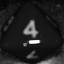
\includegraphics[width=\linewidth]{chapters/04-czytanie/figures/4processed}
        \caption{Rysunek numer2 (prawy obrazek)}
        \label{fig:4proc}
    \end{minipage}
\end{figure}


Przedstawiony algorytm został zaimplementowany w języku Python, a jego zadaniem jest identyfikacja, wycięcie i przeskalowanie obszarów zawierających obiekty zainteresowania w zdjęciach.

Zdjęcia w formacie JPEG są wczytywane za pomocą biblioteki Pillow, a następnie konwertowane do przestrzeni kolorów RGB, co zapewnia jednolitość formatów danych wejściowych.

Obrazy są przekształcane do przestrzeni barw HSV, aby oddzielić komponenty odpowiadające za barwę (H), nasycenie (S) oraz jasność (V).
Nasycenie jest następnie wygładzane przy użyciu filtra Gaussa:

--- TODO ---
jakieś cytowanie, o tym czemu filtr Gaussa?

Na podstawie komponentu nasycenia (Saturation) oraz progowania tworzona jest maska binarna, która identyfikuje obszary o wysokim nasyceniu (a więc naszą kość).

W celu usunięcia niewielkich luk w masce binarnej stosowana jest operacja zamknięcia morfologicznego z wykorzystaniem strukturalnego elementu prostokątnego z zaimportowanego modułu cv2

TODO - cytowanie o zamknięciu morfologicznym?  \\

Maska jest analizowana w celu zlokalizowania największego konturu, który określa obszar zainteresowania.
Na tej podstawie oryginalny obraz jest kadrowany w kształt prostokąta wokół obszaru zainteresowania,
a następnie przeskalowywany do wymiarów $64 \times 64$ pikseli:

Ostatecznie obraz jest konwertowany do skali szarości, co redukuje wymiarowość danych
i umożliwia naszej sieci neuronowej skupienie się na strukturze obrazu.

Dodatkowo, konwersja do skali szarości pozwala znacznie lepiej poradzić sobie z problemem odblasków,
powstających gdy kość niefortunnie ułoży się pod takim kątem, że odbija światło którejś z diód wprost do kamery.


\begin{figure}[H]
    \centering
    \begin{minipage}[t]{0.45\linewidth}
        \centering
        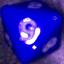
\includegraphics[width=\linewidth]{chapters/04-czytanie/figures/blask_raw}
        \caption{Rysunek numer3 (lewy obrazek)}
        \label{fig:blaskraw}
    \end{minipage}
    \hfill
    \begin{minipage}[t]{0.45\linewidth}
        \centering
        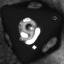
\includegraphics[width=\linewidth]{chapters/04-czytanie/figures/blask_proc}
        \caption{Rysunek numer4 (prawy obrazek)}
        \label{fig:blaskproc}
    \end{minipage}
\end{figure}



\section{Podsumowanie}

Przedstawiony algorytm przetwarzania wstępnego pozwala na skuteczne przygotowanie danych wejściowych dla modelu sztucznej inteligencji.
Automatyzuje proces identyfikacji i kadrowania obiektów zainteresowania w obrazach, co znacząco poprawia jakość danych.
Rozwiązanie zostało zaprojektowane z myślą o łatwej adaptacji do innych zastosowań wymagających podobnego przetwarzania obrazów.

